%%%%%%%%%%%%%%%%%%%%%%%%%%%%%%%%%%%%%%%%%
% Lachaise Assignment
% LaTeX Template
% Version 1.0 (26/6/2018)
%
% This template originates from:
% http://www.LaTeXTemplates.com
%
% Authors:
% Marion Lachaise & François Févotte
% Vel (vel@LaTeXTemplates.com)
%
% License:
% CC BY-NC-SA 3.0 (http://creativecommons.org/licenses/by-nc-sa/3.0/)
% 
%%%%%%%%%%%%%%%%%%%%%%%%%%%%%%%%%%%%%%%%%

%----------------------------------------------------------------------------------------
%	PACKAGES AND OTHER DOCUMENT CONFIGURATIONS
%----------------------------------------------------------------------------------------

\documentclass{article}
\usepackage{graphicx}
\usepackage{listings}
\usepackage{float}

%%%%%%%%%%%%%%%%%%%%%%%%%%%%%%%%%%%%%%%%%
% Lachaise Assignment
% Structure Specification File
% Version 1.0 (26/6/2018)
%
% This template originates from:
% http://www.LaTeXTemplates.com
%
% Authors:
% Marion Lachaise & François Févotte
% Vel (vel@LaTeXTemplates.com)
%
% License:
% CC BY-NC-SA 3.0 (http://creativecommons.org/licenses/by-nc-sa/3.0/)
% 
%%%%%%%%%%%%%%%%%%%%%%%%%%%%%%%%%%%%%%%%%

%----------------------------------------------------------------------------------------
%	PACKAGES AND OTHER DOCUMENT CONFIGURATIONS
%----------------------------------------------------------------------------------------

\usepackage{amsmath,amsfonts,stmaryrd,amssymb} % Math packages

\usepackage{enumerate} % Custom item numbers for enumerations

\usepackage[ruled]{algorithm2e} % Algorithms

\usepackage[framemethod=tikz]{mdframed} % Allows defining custom boxed/framed environments

\usepackage{listings} % File listings, with syntax highlighting
\lstset{
	basicstyle=\ttfamily, % Typeset listings in monospace font
}

%----------------------------------------------------------------------------------------
%	DOCUMENT MARGINS
%----------------------------------------------------------------------------------------

\usepackage{geometry} % Required for adjusting page dimensions and margins

\geometry{
	paper=a4paper, % Paper size, change to letterpaper for US letter size
	top=2.5cm, % Top margin
	bottom=3cm, % Bottom margin
	left=2.5cm, % Left margin
	right=2.5cm, % Right margin
	headheight=14pt, % Header height
	footskip=1.5cm, % Space from the bottom margin to the baseline of the footer
	headsep=1.2cm, % Space from the top margin to the baseline of the header
	%showframe, % Uncomment to show how the type block is set on the page
}

%----------------------------------------------------------------------------------------
%	FONTS
%----------------------------------------------------------------------------------------

\usepackage[utf8]{inputenc} % Required for inputting international characters
\usepackage[T1]{fontenc} % Output font encoding for international characters

\usepackage{XCharter} % Use the XCharter fonts

%----------------------------------------------------------------------------------------
%	COMMAND LINE ENVIRONMENT
%----------------------------------------------------------------------------------------

% Usage:
% \begin{commandline}
%	\begin{verbatim}
%		$ ls
%		
%		Applications	Desktop	...
%	\end{verbatim}
% \end{commandline}

\mdfdefinestyle{commandline}{
	leftmargin=10pt,
	rightmargin=10pt,
	innerleftmargin=15pt,
	middlelinecolor=black!50!white,
	middlelinewidth=2pt,
	frametitlerule=false,
	backgroundcolor=black!5!white,
	frametitle={Command Line},
	frametitlefont={\normalfont\sffamily\color{white}\hspace{-1em}},
	frametitlebackgroundcolor=black!50!white,
	nobreak,
}

% Define a custom environment for command-line snapshots
\newenvironment{commandline}{
	\medskip
	\begin{mdframed}[style=commandline]
}{
	\end{mdframed}
	\medskip
}

%----------------------------------------------------------------------------------------
%	FILE CONTENTS ENVIRONMENT
%----------------------------------------------------------------------------------------

% Usage:
% \begin{file}[optional filename, defaults to "File"]
%	File contents, for example, with a listings environment
% \end{file}

\mdfdefinestyle{file}{
	innertopmargin=1.6\baselineskip,
	innerbottommargin=0.8\baselineskip,
	topline=false, bottomline=false,
	leftline=false, rightline=false,
	leftmargin=2cm,
	rightmargin=2cm,
	singleextra={%
		\draw[fill=black!10!white](P)++(0,-1.2em)rectangle(P-|O);
		\node[anchor=north west]
		at(P-|O){\ttfamily\mdfilename};
		%
		\def\l{3em}
		\draw(O-|P)++(-\l,0)--++(\l,\l)--(P)--(P-|O)--(O)--cycle;
		\draw(O-|P)++(-\l,0)--++(0,\l)--++(\l,0);
	},
	nobreak,
}

% Define a custom environment for file contents
\newenvironment{file}[1][File]{ % Set the default filename to "File"
	\medskip
	\newcommand{\mdfilename}{#1}
	\begin{mdframed}[style=file]
}{
	\end{mdframed}
	\medskip
}

%----------------------------------------------------------------------------------------
%	NUMBERED QUESTIONS ENVIRONMENT
%----------------------------------------------------------------------------------------

% Usage:
% \begin{question}[optional title]
%	Question contents
% \end{question}

\mdfdefinestyle{question}{
	innertopmargin=1.2\baselineskip,
	innerbottommargin=0.8\baselineskip,
	roundcorner=5pt,
	nobreak,
	singleextra={%
		\draw(P-|O)node[xshift=1em,anchor=west,fill=white,draw,rounded corners=5pt]{%
		Question \theQuestion\questionTitle};
	},
}

\newcounter{Question} % Stores the current question number that gets iterated with each new question

% Define a custom environment for numbered questions
\newenvironment{question}[1][\unskip]{
	\bigskip
	\stepcounter{Question}
	\newcommand{\questionTitle}{~#1}
	\begin{mdframed}[style=question]
}{
	\end{mdframed}
	\medskip
}

%----------------------------------------------------------------------------------------
%	WARNING TEXT ENVIRONMENT
%----------------------------------------------------------------------------------------

% Usage:
% \begin{warn}[optional title, defaults to "Warning:"]
%	Contents
% \end{warn}

\mdfdefinestyle{warning}{
	topline=false, bottomline=false,
	leftline=false, rightline=false,
	nobreak,
	singleextra={%
		\draw(P-|O)++(-0.5em,0)node(tmp1){};
		\draw(P-|O)++(0.5em,0)node(tmp2){};
		\fill[black,rotate around={45:(P-|O)}](tmp1)rectangle(tmp2);
		\node at(P-|O){\color{white}\scriptsize\bf !};
		\draw[very thick](P-|O)++(0,-1em)--(O);%--(O-|P);
	}
}

% Define a custom environment for warning text
\newenvironment{warn}[1][Warning:]{ % Set the default warning to "Warning:"
	\medskip
	\begin{mdframed}[style=warning]
		\noindent{\textbf{#1}}
}{
	\end{mdframed}
}

%----------------------------------------------------------------------------------------
%	INFORMATION ENVIRONMENT
%----------------------------------------------------------------------------------------

% Usage:
% \begin{info}[optional title, defaults to "Info:"]
% 	contents
% 	\end{info}

\mdfdefinestyle{info}{%
	topline=false, bottomline=false,
	leftline=false, rightline=false,
	nobreak,
	singleextra={%
		\fill[black](P-|O)circle[radius=0.4em];
		\node at(P-|O){\color{white}\scriptsize\bf i};
		\draw[very thick](P-|O)++(0,-0.8em)--(O);%--(O-|P);
	}
}

% Define a custom environment for information
\newenvironment{info}[1][Info:]{ % Set the default title to "Info:"
	\medskip
	\begin{mdframed}[style=info]
		\noindent{\textbf{#1}}
}{
	\end{mdframed}
}
 % Include the file specifying the document structure and custom commands

%----------------------------------------------------------------------------------------
%	ASSIGNMENT INFORMATION
%----------------------------------------------------------------------------------------

\title{Random Forest Fires:\\Modeling Wildfire Probability with Weather} % Title of the assignment

\author{Matt Elser\\ \texttt{elserm@gmail.com}} % Author name and email address

\date{\today} % University, school and/or department name(s) and a date

%----------------------------------------------------------------------------------------

\begin{document}

\maketitle % Print the title

%----------------------------------------------------------------------------------------
%	INTRODUCTION
%----------------------------------------------------------------------------------------

\section*{Introduction} % Unnumbered section

Lorem ipsum dolor sit amet, consectetur adipiscing elit. Praesent porttitor arcu luctus, imperdiet urna iaculis, mattis eros. Pellentesque iaculis odio vel nisl ullamcorper, nec faucibus ipsum molestie. Sed dictum nisl non aliquet porttitor. Etiam vulputate arcu dignissim, finibus sem et, viverra nisl. Aenean luctus congue massa, ut laoreet metus ornare in. Nunc fermentum nisi imperdiet lectus tincidunt vestibulum at ac elit. Nulla mattis nisl eu malesuada suscipit.

\section{Requirements} % Numbered section

Running the code requires the following modules:
\begin{itemize}
	\item \lstinline|pandas|
	\item \lstinline|numpy|
	\item \lstinline|sklearn|
	\item \lstinline|requests| - for accessing FCC area information API
	\item \lstinline|plotly| - for creating graphs of geographic areas
	\item \lstinline|kaleido| - required for plotly to write graphs to images
\end{itemize}


As well as the code and data available at https://github.com/mattelser/randomForestFires. The tool \lstinline|ffmpeg| was used to combine graphs into an animation, viewable at the aforementioned github link. All work was done on a unix system and no validation was feasible on windows.  
%------------------------------------------------

\section{Data Gathering}

Weather data is readily available from the National Climatic Data Center (NCDC) and the National Oceanic and Atmospheric Administration (NOAA), and wildfire data is made available by the California Department of Forestry and Fire Protection (CalFire), however obtaining sufficient data in a usable form still proved challenging. Raw data from NOAA
\footnote{https://www.ncdc.noaa.gov/cdo-web/search} (available in \lstinline|/rawData/weather|
) had to be obtained through multiple manually-clicked requests, as no API existed to query and a limit on request size meant several requests had to be made per year of data. CalFire makes their data available via "Redbook" pdfs
\footnote{https://www.fire.ca.gov/stats-events/}
, from which the contents of tables was manually extracted using a tool called \lstinline|Tabula|. The fire data is only by county, while the weather data was by station, which had no county attributed. Separately, a collection of latitudes and longitudes was obtained (again from NCDC/NOAA) for each station. This allowed for obtaining county via an API made available by the Federal Communications Comission (FCC)
\footnote{https://geo.fcc.gov/api/census/\#!/area/get\_area}
, which accepts a latitude/longitude pair and returns geographic information. Included in this information is both county name and Federal Information Processing Standards (FIPS) code, which was one key part in graphing information by county. The second key part to graphing by county is pairing each FIPS code with a polygonal outline of that county (defined by points of latitude/longitude). This was available via an example in the documentation for the graphing module \lstinline|plotly|
\footnote{https://raw.githubusercontent.com/plotly/datasets/master/geojson-counties-fips.json} in the form of a "geojson" file defining the shape of all counties in the US. A paired-down version of this geojson file containing only California is available in \lstinline|//CalCountyGeoJson.json|.

\section{Code Description}
The bulk of the code centers around joining, clustering, cleaning, bucketing, and extrapolating from the data. This includes all data gathering steps mentioned above, other than those explicitly mentioned as being manual (requesting weather data and extracting tables from CalFire pdfs). The data pipeline starts with these manually extracted data files, then develops them in stages, "baking" the results out in between. First, 
\lstinline|bakeData.py| takes all the per-station-per-date observations from
\lstinline|\cleanedData| and generates average per-county data for each date, as well as a rolling average of temperature and the recent presence of precipitation per county. Measurements are also bucketed for better usability in a random forest model. Once we have observations per county per date, we join the fire data, which begins as various fields per-fire (notably, county, start date, and date of containment). We end up with a data frame where each row is an observation of one county on a given day, including weather and how many fires are burning that day. A description of each action is printed to stdout:
\begin{figure}[h]
	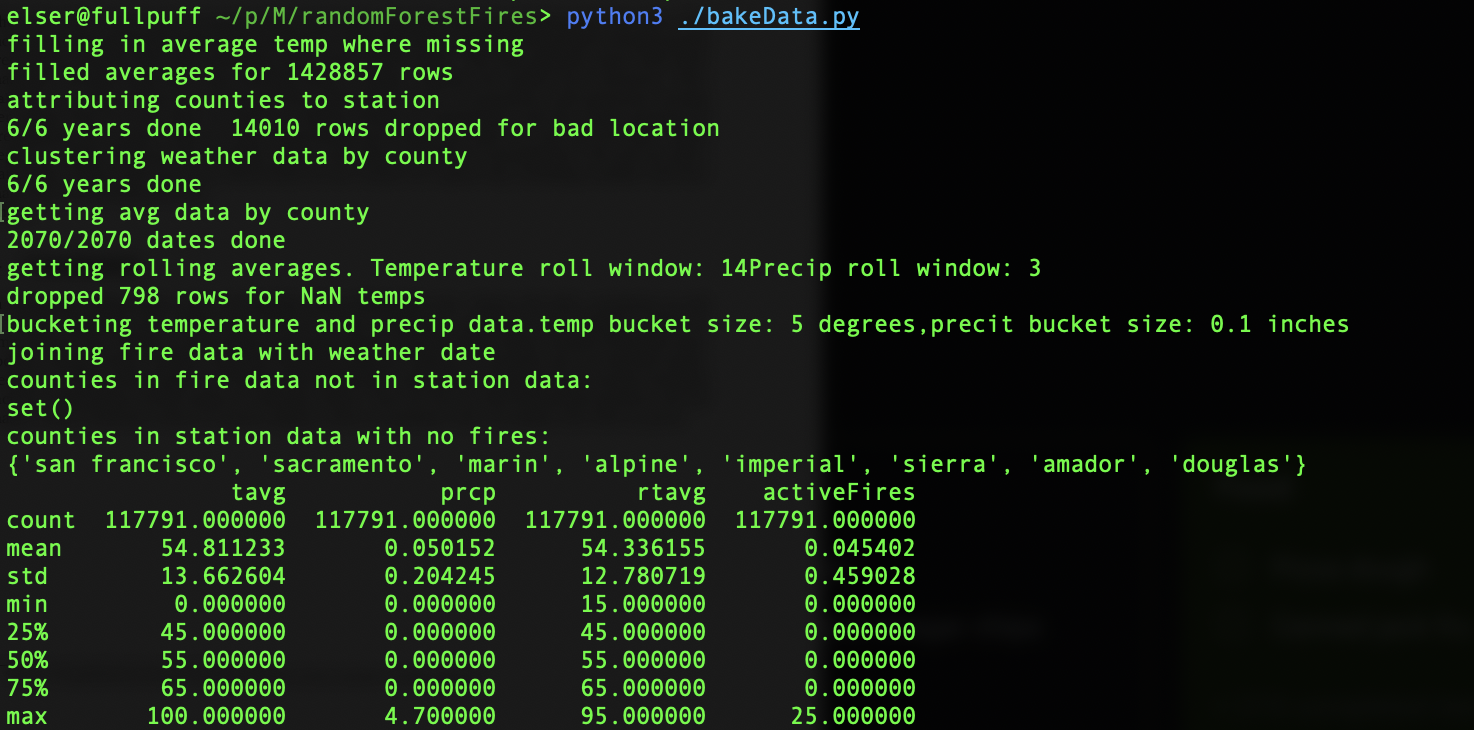
\includegraphics[width=\linewidth]{images/bakeDataScreenshot.png}
\end{figure}
\\
This is the data that feeds the model. A \lstinline|RandomForestClassifier| is fed per county per day observations of average temperature, precipitation level, a rolling average of temperature, whether there has recently been precipitation, and what county these observations were in. Notably, date is not given to the model, even though these observations are per-date, because dates do not contribute to fires and should therefore not be part of the decision trees generated by our random forest model. The target is whether there is a fire in that county. Initial runs of the model were very good at predicting when/where there would not be a fire, and mediocre at predicting when/where a fire would occur. Fires are relatively rare in the dataset, so it makes sense that they would not be predicted often, however in this case false negatives could be catastrophic and therefore reweighting of the model was necessary. Observations with fires were given a higher weight, and that weight was further scaled by the number of fires in the county. Here are the results of the model before weighting:
\begin{figure}[H]
	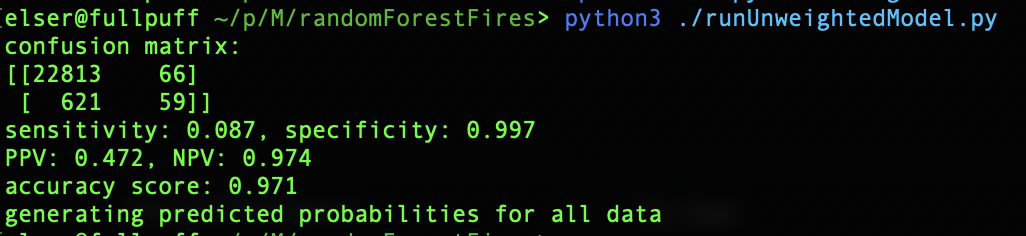
\includegraphics[width=\linewidth]{images/runUnweightedModelScreenshot.png}
\end{figure}
And after reweighting, the sensitivity improves nearly tenfold. Our positive predictive value decreases, however the cost of a false positive is extremely low in comparison to a false negative, so our gains seem more than worth it. 
\begin{figure}[H]
	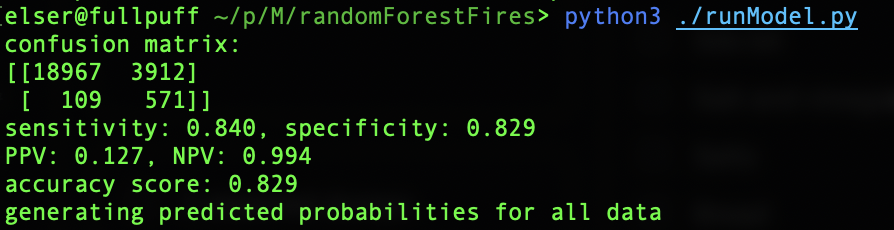
\includegraphics[width=\linewidth]{images/runModelScreenshot.png}
\end{figure}
Using this model, we can generate a predicted probability of having a fire in each county for each day, given the weather data. These predicted probabilities were generated for all per-county weather observations, allowing the creation of graphs like these:

\begin{figure}[h!]
	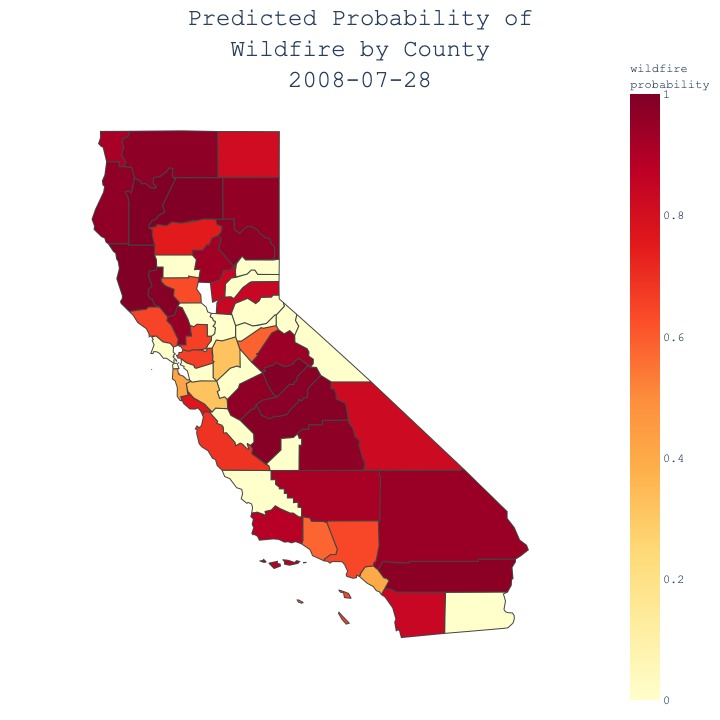
\includegraphics[width=.75\linewidth]{images/animGraph_0189.jpg}
\end{figure}
\begin{figure}[h!]
	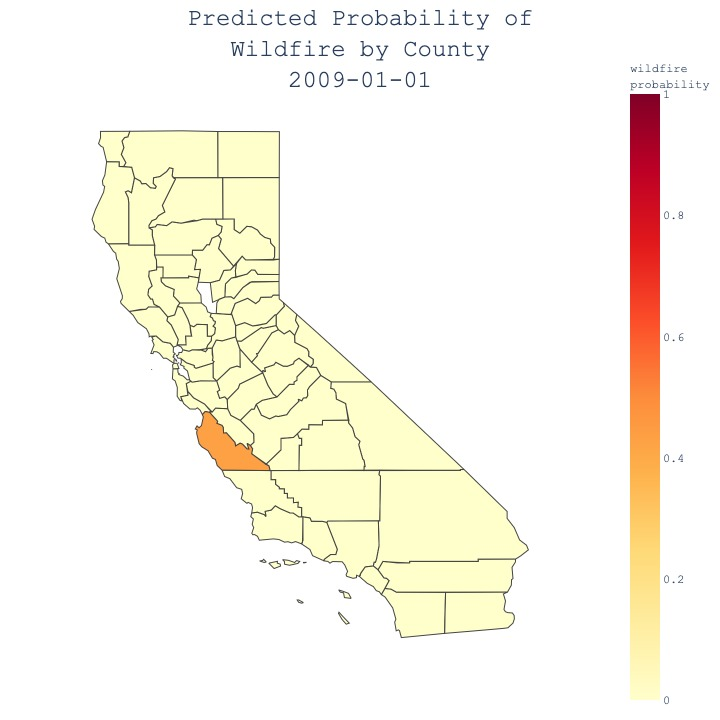
\includegraphics[width=.5\linewidth]{images/animGraph_0346.jpg}
	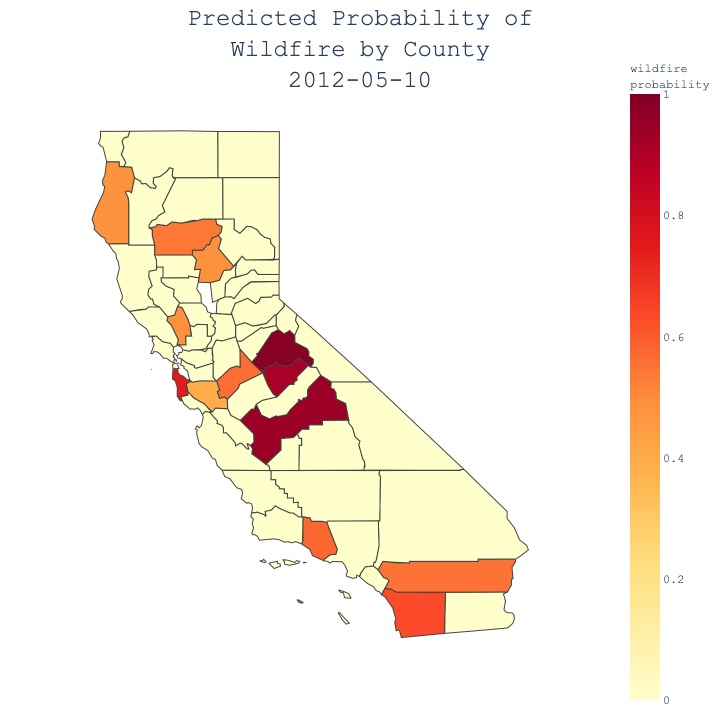
\includegraphics[width=.5\linewidth]{images/animGraph_1571.jpg}
\end{figure}

Such graphs were created using \lstinline|plotly|, which can generate choropleths using the generated data and geojson described above. Each observation was given a probability and graphed, which, when combined using \lstinline|ffmpeg|, create an animation showing predicted probability of fire by county over time. This animation can be viewed at the github repository mentioned in the Requirements section, or can be generated (assuming the required data has been baked out by \lstinline|bakeData.py| then \lstinline|runModel.py|) by running \lstinline|animPlotCounties.py| then \lstinline|convertFramesToGraph.sh| .

%------------------------------------------------

\section{Conclusion}

In malesuada ullamcorper urna, sed dapibus diam sollicitudin non. Donec elit odio, accumsan ac nisl a, tempor imperdiet eros. Donec porta tortor eu risus consequat, a pharetra tortor tristique. Morbi sit amet laoreet erat. Morbi et luctus diam, quis porta ipsum. Quisque libero dolor, suscipit id facilisis eget, sodales volutpat dolor. Nullam vulputate interdum aliquam. Mauris id convallis erat, ut vehicula neque. Sed auctor nibh et elit fringilla, nec ultricies dui sollicitudin. Vestibulum vestibulum luctus metus venenatis facilisis. Suspendisse iaculis augue at vehicula ornare. Sed vel eros ut velit fermentum porttitor sed sed massa. Fusce venenatis, metus a rutrum sagittis, enim ex maximus velit, id semper nisi velit eu purus.

\end{document}
